% \svnInfo $Id: Tutorium3-Dijkstra.tex 3 2011-05-18 11:22:28Z felixlindemann $
	\NeedsTeXFormat{LaTeX2e}
	\documentclass{scrartcl}
	 
	\usepackage[
		%%answers, 						%LösungFürStudenten
		%MusterLoesung,			%Musterlösung
		isGruppenarbeit,		%Gruppenarbeit
		GiveLines,					%Raum für Antworten
		GivePoints,					%Kästen zur Benotung
		Inhaltsverzeichnis 	%Inhaltsverzeichnis
	]
	{Klausur}
	%	  
	\setKlausurVersionDatum{\today~\thistime~Uhr}
	\setKlausurTyp{Tutorium} % just a
	\setKlausurName{\KlausurTyp~No.3 - Dijkstra}
	\setKlausurFach{Transportwirtschaft Sommersemester 2011}
	\setKlausurDatum{18. April 2011 09:30 Uhr}
	\setKlausurProfessor{Name des Professors}
	 \Huge
	\bibliography{bib/literature}
	\addtocategory{primary}{ Neumann.2004,Kathofer.2008.740,Hillier.2002,Heinrich.2007,Gal.1992.741,Domschke.2007,Domschke.2005} 
	\addtocategory{secondary}{Arnold.2005,Furmans.2008,MullerMerbach.1992.742,Feige.2008}
	\begin{document}
	\sffamily\onehalfspacing
%Falls kein Subversion verwendet wird, kann diese Zeile ggf. manuelle angepasst werden.
\svnInfo $Id: Tutorium3-Dijkstra.tex 3 2011-05-18 11:22:28Z felixlindemann $
	 \TitleTutoriumA
	%%
	 	\Aufgabe %1
					 {Theoretische Fragen}
					 {Tipp: Zur Bearbeitung der folgenden Aufgaben ist ein Blick in die empfohlene Literatur 
					 sowie die Vorlesungsunterlagen notwendig!} 
					 % \svnInfo $Id: a1a.tex 2 2011-05-18 10:04:02Z felixlindemann $

\TeilAufgabe
				 {Auf \url{http://de.wikipedia.org/wiki/Dijkstra-Algorithmus} hei�t es:\\
"`\emph{Der Algorithmus von Dijkstra [\ldots] ist ein Algorithmus aus der Klasse der Greedy-Algorithmen 
und dient der Berechnung eines k�rzesten Pfades zwischen einem Startknoten 
und einem beliebigen Knoten in einem kantengewichteten Graphen.}"'\\
Diskutieren Sie, ob der Algorithmus von Dijkstra tats�chlich zur Familie der Greedy-Heuristiken geh�rt.\\
Hinweis: Definieren Sie dazu zun�chst den Begriff der Greedy Heuristik.}
				 {6}
\KlausurAntwortLinien{6}
\KlausurErgebnis{Richtig, Erl�uterungen siehe Tutorium}
\KlausurMusterLoesung{Richtig/ja(1p), eine Greedyheuristik w�hlt \emph{gierig} die lokal beste L�sung aus(1p), ohne dabei auf das Gesamtoptimum zu achten.(1p)
Der Alg. von Dijkstra w�hlt auch das lokale Optimum aus.(1p) Da ein gesamt-k�rzester Weg immer aus Teil-k�rzesten Wegen besteht,(1p)
kann der Alg. von Dijkstra als Sonderfall interpretiert werden.(1p)} 
\KlausurKorrekturhinweis{je Aspekt 1p, Gro�z�gig bewerten } 
\KlausurErlaeuterung{-}
%
\TeilAufgabe
				 {Gehen Sie davon aus, dass in einem beliebigen symmetrischen Netzwerk 5 Knoten ($A-E$) existieren.\\
Diskutieren Sie, ob der k�rzeste Weg von $A$ nach $E$ im Netz identisch mit dem Weg von $E$ nach $A$ ist, 
wenn beide Wege mit dem \emph{Algorithmus von Dijkstra} berechnet werden.\\
Illustrieren Sie Ihre Ausf�hrungen mit einer Skizze.}
				 {4}
\KlausurAntwortLinien{4}
\KlausurAntwortKasten{4cm}
\KlausurErgebnis{Ja, beide Wege sind gleich-lang, Erl�uterungen siehe Tutorium}
\KlausurMusterLoesung{Ja, beide Wege sind gleich-lang.(1p) Im Falle eines asymmetrischen (1P) Netzwerks kann sich eine andere Route (1p) ergeben.} 
\KlausurKorrekturhinweis{F�r korrekte Antwort 3P, 1p Skizze} 
\KlausurErlaeuterung{-}
%%
%\ 
\ifisAufgabenstellung{\newpage}
\TeilAufgabe
				 {Was ist die Bedeutung von $Q$ im Dijkstra-Tableau? }
				 {2}
\KlausurAntwortLinien{6}
\KlausurErgebnis{Richtig, Erl�uterungen siehe Tutorium}
\KlausurMusterLoesung{Die Menge $Q$ ist eine sortierte Liste der erreichbaren Knoten (1p).
 Die Knoten sind aufsteigend sortiert anzugeben (1p). \\Alternativ: Das Element mit niedrigstem Kostenwert steht vorne.(1p)   }
\KlausurKorrekturhinweis{je Aspekt 1p} 
\KlausurErlaeuterung{-}
% 
\TeilAufgabe
				 {Wieviele Knoten werden beim Dijkstra-Algorithmus bei der Ermittlung von k�rzesten Wegen
				 je Iteration ausgew�hlt?}
				 {1}
\KlausurAntwortLinien{2}
\KlausurErgebnis{genau 1 Knoten}
\KlausurMusterLoesung{genau 1 Knoten(1p)  } 
\KlausurKorrekturhinweis{1p} 
\KlausurErlaeuterung{-}
%  
	 	\newpage% \svnInfo $Id: a2a.tex 2 2011-05-18 10:04:02Z felixlindemann $
\Aufgabe %1
				 {Korrektur Fragen}
				 {\ifisAufgabenstellung{Im Folgenden erhalten Sie den K�rzeste-Wege-L�sungsvorschlag 
				 (Tabelle \ref{tbl.SolutionStudent}) eines Kommilitonen f�r nachstehenden Graphen.
				 \input{grafik/netzdijkstra}
				 % \svnInfo $Id: a2TableStud.tex 2 2011-05-18 10:04:02Z felixlindemann $
\begin{table}[H]\centering
\begin{tabular}{|c||cc|cc|cc|cc|cc|cc|cc|}
\hline
 & \multicolumn{2}{|c|}{1}   & \multicolumn{2}{|c|}{2} &  \multicolumn{2}{|c|}{3} 
 & \multicolumn{2}{|c|}{4} &  \multicolumn{2}{|c|}{5}    & \multicolumn{2}{|c|}{6} &  \multicolumn{2}{|c|}{7}\\  
 & d & p & d & p & d & p & d & p & d & p & d & p & d & p\\\hline\hline
1 & 0 & - & 0 & - & 0 & - & 0 & - & 0 & - & 0 & - & 0 & -\\\hline
2 & $\infty$ & - & 4 & 1 & 4 & 1 & 4 & 1 & 4 & 1 & 4 & 1 & 4 & 1\\\hline
3 & $\infty$ & - & $\infty$ & 1 & 7 & 2 & 7 & 2 & 7 & 2 & 7 & 2 & 7 & 2\\\hline
4 & $\infty$ & - & $\infty$ & - & 8 & 2 & 8 & 2 & 8 & 2 & 8 & 2 & 8 & 2\\\hline
5 & $\infty$ & - & $\infty$ & - & 6 & 2 & 6 & 2 & 6 & 2 & 6 & 2 & 6 & 2\\\hline
6 & $\infty$ & - & $\infty$ & - & $\infty$ & - & 13 & 5 & 12 & 4 & 12 & 4 & 12 & 4\\\hline\hline
$Q$ & \multicolumn{2}{|c|}{ }    & \multicolumn{2}{|c|}{ }    & \multicolumn{2}{|c|}{ }    & \multicolumn{2}{|c|}{ }   & \multicolumn{2}{|c|}{ }   & \multicolumn{2}{|c|}{ }    & \multicolumn{2}{|c|}{ }   
\\\hline
\end{tabular}
\caption{L�sung Ihres Kommilitonen}
\label{tbl.SolutionStudent}
\end{table}}	~			 
				 }
\TeilAufgabe{Stellen Sie fest, ob Ihr Kommilitone richtig gerechnet hat. Berechnen Sie dazu 
				 eine eigene L�sung.
				 \ifisAufgabenstellung{ Nutzen Sie f�r Ihre L�sung Tabelle \ref{tbl.SolutionYou}!}}
				 {15}
				 \ifisAufgabenstellung{
% \svnInfo $Id: a2TableYour.tex 2 2011-05-18 10:04:02Z felixlindemann $
\begin{table}[H]\centering
\begin{tabular}{|c||p{0.75cm}|p{0.75cm}|p{0.75cm}|p{0.75cm}|p{0.75cm}|p{0.75cm}|p{0.75cm}|p{0.75cm}|p{0.75cm}|p{0.75cm}|p{0.75cm}|p{0.75cm}|p{0.75cm}|p{0.75cm}|}
\hline
 & \multicolumn{2}{|c|}{1}   & \multicolumn{2}{|c|}{2} &  \multicolumn{2}{|c|}{3} 
 & \multicolumn{2}{|c|}{4} &  \multicolumn{2}{|c|}{5}    & \multicolumn{2}{|c|}{6} &  \multicolumn{2}{|c|}{7}\\  
 & d & p & d & p & d & p & d & p & d & p & d & p & d & p\\\hline\hline
1 &   &   &   &   &   &   &   &   &   &   &   &   &   &  \\[1em]\hline
2 &   &   &   &   &   &   &   &   &   &   &   &   &   &  \\[1em]\hline
3 &   &   &   &   &   &   &   &   &   &   &   &   &   &  \\[1em]\hline
4 &   &   &   &   &   &   &   &   &   &   &   &   &   &  \\[1em]\hline
5 &   &   &   &   &   &   &   &   &   &   &   &   &   &  \\[1em]\hline
6 &   &   &   &   &   &   &   &   &   &   &   &   &   &  \\[1em]\hline
$Q$ & \multicolumn{2}{|c|}{ }    & \multicolumn{2}{|c|}{ }    & \multicolumn{2}{|c|}{ }    & \multicolumn{2}{|c|}{ }   & \multicolumn{2}{|c|}{ }   & \multicolumn{2}{|c|}{ }    & \multicolumn{2}{|c|}{ }   
\\[1em]\hline
\end{tabular}
\caption{Tragen Sie hier Ihre L�sung ein.}
\label{tbl.SolutionYou}
\end{table}	}	
\KlausurErgebnis{% \svnInfo $Id: a2TableML.tex 2 2011-05-18 10:04:02Z felixlindemann $
\begin{table}[H]\centering
\begin{tabular}{|c||cc|cc|cc|cc|cc|cc|cc|}
\hline
 & \multicolumn{2}{|c|}{1}   & \multicolumn{2}{|c|}{2} &  \multicolumn{2}{|c|}{3} 
 & \multicolumn{2}{|c|}{4} &  \multicolumn{2}{|c|}{5}    & \multicolumn{2}{|c|}{6} &  \multicolumn{2}{|c|}{7}\\  
 & d & p & d & p & d & p & d & p & d & p & d & p & d & p\\\hline\hline
1 & 0 & - & 0 & - & 0 & - & 0 & - & 0 & - & 0 & - & 0 & -\\\hline
2 & $\infty$ & - & 4 & 1 & 4 & 1 & 4 & 1 & 4 & 1 & 4 & 1 & 4 & 1\\\hline
3 & $\infty$ & - & 8 & 1 & 7 & 2 & 7 & 2 & 7 & 2 & 7 & 2 & 7 & 2\\\hline
4 & $\infty$ & - & $\infty$ & - & 8 & 2 & 8 & 2 & 8 & 2 & 8 & 2 & 8 & 2\\\hline
5 & $\infty$ & - & $\infty$ & - & $\infty$ & - & 14 & 3 & 11 & 4 & 11 & 4 & 11 & 4\\\hline
6 & $\infty$ & - & $\infty$ & - & $\infty$ & - & $\infty$ & - & 12 & 4 & 12 & 4 & 12 & 4\\\hline\hline
$Q$ & \multicolumn{2}{|c|}{$\left\{1\right\}$}    & \multicolumn{2}{|c|}{$\left\{2,3\right\}$}    & \multicolumn{2}{|c|}{$\left\{3,4\right\}$}    & \multicolumn{2}{|c|}{$\left\{4,5\right\}$}   & \multicolumn{2}{|c|}{$\left\{5,6\right\}$}   & \multicolumn{2}{|c|}{$\left\{6\right\}$}    & \multicolumn{2}{|c|}{$\left\{-\right\}$}   
\\\hline
\end{tabular}
\caption{L�sung}
\label{tbl.Solution}
\end{table}		}
\KlausurMusterLoesung{% \svnInfo $Id: a2TableML.tex 2 2011-05-18 10:04:02Z felixlindemann $
\begin{table}[H]\centering
\begin{tabular}{|c||cc|cc|cc|cc|cc|cc|cc|}
\hline
 & \multicolumn{2}{|c|}{1}   & \multicolumn{2}{|c|}{2} &  \multicolumn{2}{|c|}{3} 
 & \multicolumn{2}{|c|}{4} &  \multicolumn{2}{|c|}{5}    & \multicolumn{2}{|c|}{6} &  \multicolumn{2}{|c|}{7}\\  
 & d & p & d & p & d & p & d & p & d & p & d & p & d & p\\\hline\hline
1 & 0 & - & 0 & - & 0 & - & 0 & - & 0 & - & 0 & - & 0 & -\\\hline
2 & $\infty$ & - & 4 & 1 & 4 & 1 & 4 & 1 & 4 & 1 & 4 & 1 & 4 & 1\\\hline
3 & $\infty$ & - & 8 & 1 & 7 & 2 & 7 & 2 & 7 & 2 & 7 & 2 & 7 & 2\\\hline
4 & $\infty$ & - & $\infty$ & - & 8 & 2 & 8 & 2 & 8 & 2 & 8 & 2 & 8 & 2\\\hline
5 & $\infty$ & - & $\infty$ & - & $\infty$ & - & 14 & 3 & 11 & 4 & 11 & 4 & 11 & 4\\\hline
6 & $\infty$ & - & $\infty$ & - & $\infty$ & - & $\infty$ & - & 12 & 4 & 12 & 4 & 12 & 4\\\hline\hline
$Q$ & \multicolumn{2}{|c|}{$\left\{1\right\}$}    & \multicolumn{2}{|c|}{$\left\{2,3\right\}$}    & \multicolumn{2}{|c|}{$\left\{3,4\right\}$}    & \multicolumn{2}{|c|}{$\left\{4,5\right\}$}   & \multicolumn{2}{|c|}{$\left\{5,6\right\}$}   & \multicolumn{2}{|c|}{$\left\{6\right\}$}    & \multicolumn{2}{|c|}{$\left\{-\right\}$}   
\\\hline
\end{tabular}
\caption{L�sung}
\label{tbl.Solution}
\end{table} } 
\KlausurKorrekturhinweis{je Korrekter Iteration jeweils 
1p f�r korrektes $Q$, 
1p f�r korrekte Entfernungen
Max. 14p.} 
\KlausurErlaeuterung{-}
\TeilAufgabe{Erkl�ren Sie Ihrem Kommilitonen die gemachten Fehler.}
				 {3}
\KlausurAntwortLinien{4}
\KlausurErgebnis{\begin{enumerate}
	\item $Q$ wurde pauschal nicht angegeben
	\item $\infty$ in Iteration 2 muss eine 8 sein
	\item Die Strecke von $v_2$ nach $v_5$ die in Iteration 3 verwendet wurde 
				existiert nur in der Gegenrichtung.
\end{enumerate}}
\KlausurMusterLoesung{\begin{enumerate}
	\item $Q$ wurde pauschal nicht angegeben
	\item Die Strecke von $v_2$ nach $v_5$ die in Iteration 3 verwendet wurde 
				existiert nur in der Gegenrichtung.
\end{enumerate} } 
\KlausurKorrekturhinweis{jeweils 1p Max 2} 
\KlausurErlaeuterung{-}
\TeilAufgabe{Erkl�ren Sie Ihrem Kommilitonen wie aus Ihrem Dijkstra Tableau 
					 \ifisAufgabenstellung{(Tabelle \ref{tbl.SolutionYou})}
						der k�rzeste Weg sowie die L�nge von Knoten $v_1$ zu Knoten $v_5$ abgelesen werden kann. 
						Geben Sie dabei auch den Weg, sowie die Gesamtl�nge an!}
				 {5}
\KlausurAntwortLinien{4}
\KlausurErgebnis{Rekursiv - Siehe Tutorium}
\KlausurMusterLoesung{Rekursiv(1p): Der Weg vom Startknoten zu Knoten $v_5$ betr�gt 11 Einheiten(1p) (Zeile 5 Iteration 7 Spalte d). Der Vorg�nger von Knoten $v_5$ ist $v_4$(Zeile 5 Iteration 7 Spalte p). Der Vorg�nger von Knoten $v_4$ ist $v_2$ und der Vorg�nger von $v_2$ ist $v_1$.(2p) 
Daraus folgt das der Weg vom Startknoten zum Knoten $v_5$ lautet: $v_1\rightarrow v_2\rightarrow v_4\rightarrow  v_5$(1p)  } 
\KlausurKorrekturhinweis{Siehe Musterl�sung.} 
\KlausurErlaeuterung{-} 
	 	\newpage
	 	\Aufgabe{Fallstudie}
					 {\ifisAufgabenstellung{
					 \minisec{Hintergrundinformationen:} 
					 Als Logistikdienstleister prüfen Sie für einen Kunden aus Eching (ECH) die Routen
					 zu seinen Kunden. Benutzen Sie für Ihre Planung die vereinfachte Karte (Abbildung \ref{map.MUC}).
					 In dieser Karte sind die Kundenstandorte (DAH = Dachau, FFB = Fürstenfeldbruck, GRA = Grafing, ICK = Icking,
					 MSC = Markt Schwaben, MUC = München, SAU = Sauerlach, WES = Weßling) Rot und Wegpunkte (A-R) Blau markiert worden.
					 Die Länge einer Strecke ist in [km] in einem Kreis auf der jeweiligen Strecke gegeben.\\
					 In den Tabellen \ref{tbl.dijkstra.A} und \ref{tbl.dijkstra.B} sind Ihnen die ersten 19 
					 Iterationen des Dijkstra Tableaus gegeben. 
					 % \svnInfo $Id: a3Karte.tex 2 2011-05-18 10:04:02Z felixlindemann $
\begin{figure}[H]\centering
\begin{tikzpicture}[scale=0.1]
\node[inner sep=0pt] at (70,46) {%
        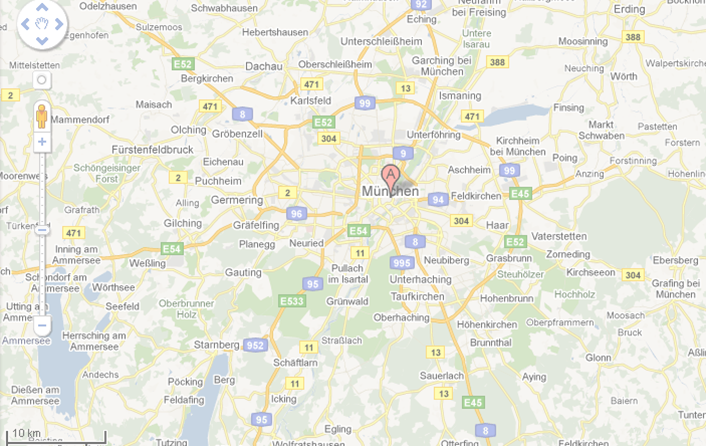
\includegraphics[scale =0.64]{grafik/MUC1.png}%
    };% 
		\tikzstyle{tikzNodeLocation}=[fill=red,draw,circle,inner sep=1pt,font=\sf \tiny]
		\tikzstyle{tikzNode}=[pin distance=2cm,fill=blue,draw,circle,inner sep=1.5pt,font=\sf \tiny]
		\tikzstyle{tikzNodeLength}=[fill=white,draw,circle,inner sep=1pt,font=\sf \tiny]

\node[tikzNodeLocation] (MUC) at (79,50) {  MUC};
\node[tikzNodeLocation] (FFB) at (28,59) {FFB};
\node[tikzNodeLocation] (DAH) at (56,77) {DAH};
\node[tikzNodeLocation] (ECH) at (84,90) {ECH};
\node[tikzNodeLocation] (MSC) at (120,63) {MSC};
\node[tikzNodeLocation] (GRA) at (136,30) {GRA};
\node[tikzNodeLocation] (SAU) at (88,13) {SAU};
\node[tikzNodeLocation] (ICK) at (56,8) {ICK};
\node[tikzNodeLocation] (WES) at (29,36) {WES};
%\tikz[pin distance=2cm]  
	\node[tikzNode, pin=180:\tiny\sffamily \bfseries A] (78A8) at (43,72) {};
\node[tikzNode,pin=-90:\tiny\sffamily \bfseries B ] (04A99) at (52,47) {};
%\node[tikzNode,label=180:\tiny\sffamily  WES ] (06A99) at (51,52) {};
\node[tikzNode,pin=200:\tiny\sffamily  C ] (09A99) at (57,64) {};
\node[tikzNode,pin=80:\tiny\sffamily \bfseries D ] (10A99) at (63,66) {};
\node[tikzNode,pin=30:\tiny\sffamily \bfseries E ] (13A99) at (85,68) {};
\node[tikzNode,pin=0:\tiny\sffamily \bfseries F ] (17A99) at (105,51) {};
\node[tikzNode,pin=-90:\tiny\sffamily \bfseries G ] (18A99) at (103,42) {};
\node[tikzNode,pin=-90:\tiny\sffamily \bfseries H ] (04A9X) at (82,27) {};
\node[tikzNode,pin=-45:\tiny\sffamily \bfseries I ] (21A99) at (90,25) {};
\node[tikzNode,pin=-90:\tiny\sffamily\bfseries  J ] (B11G) at (67,29) {};
\node[tikzNode,pin=0:\tiny\sffamily\bfseries  K ] (B11S) at (59,17) {};
\node[tikzNode,pin=-90:\tiny\sffamily\bfseries L ] (04A95) at (53,22) {};
\node[tikzNode,pin=0:\tiny\sffamily \bfseries M ] (01MR) at (80,58) {};
\node[tikzNode,pin=30:\tiny\sffamily\bfseries  N ] (03MR) at (86,50) {};
\node[tikzNode,pin=0:\tiny\sffamily \bfseries O ] (04MR) at (84,43) {};
\node[tikzNode,pin=240:\tiny\sffamily\bfseries  P ] (05MR) at (78,42) {};
\node[tikzNode,pin=120:\tiny\sffamily \bfseries Q ] (07MR) at (68,43) {};
%\node[tikzNode,label=180:\tiny\sffamily  WES ] (09MR) at (71,51) {};
\node[tikzNode,pin=180:\tiny\sffamily\bfseries  R ] (10MR) at (72,56) {};
%\node[tikzNode,label=180:\tiny\sffamily  WES ] (05A9X) at (86,25) {};
%

		\begin{scope} [line width=0.2mm]
			\path[-] (MUC) edge        node[tikzNodeLength] {9} (01MR);
%\path[-] (MUC) edge        node[tikzNodeLength] {9} (01MR);
\path[-] (MUC) edge        node[tikzNodeLength] {7} (03MR);
%\path[-] (MUC) edge        node[tikzNodeLength] {8} (04MR);
\path[-] (MUC) edge        node[tikzNodeLength] {10} (05MR);
\path[-] (MUC) edge        node[tikzNodeLength] {13} (07MR);
%\path[-] (MUC) edge        node[tikzNodeLength] {10} (09MR);
\path[-] (MUC) edge        node[tikzNodeLength] {10} (10MR);
\path[-] (FFB) edge        node[tikzNodeLength] {21} (WES);
\path[-] (FFB) edge        node[tikzNodeLength] {10} (78A8);
%\path[-] (FFB) edge        node[tikzNodeLength] {12} (06A99);
\path[-] (FFB) edge        node[tikzNodeLength] {12} (04A99); %neu Lindemann
\path[-] (DAH) edge        node[tikzNodeLength] {22} (ECH);
\path[-] (DAH) edge        node[tikzNodeLength] {9} (78A8);
\path[-] (DAH) edge        node[tikzNodeLength] {11} (10A99);
\path[-] (ECH) edge        node[tikzNodeLength] {7} (13A99);
\path[-] (MSC) edge        node[tikzNodeLength] {25} (GRA);
\path[-] (MSC) edge        node[tikzNodeLength] {9} (17A99);
\path[-] (GRA) edge        node[tikzNodeLength] {20} (18A99);
\path[-] (SAU) edge        node[tikzNodeLength] {29} (ICK);
\path[-] (SAU) edge        node[tikzNodeLength] {7} (21A99);
%\path[-] (SAU) edge        node[tikzNodeLength] {6} (05A9X);
\path[-] (ICK) edge        node[tikzNodeLength] {4} (B11S);
\path[-] (WES) edge        node[tikzNodeLength] {10} (04A99);
\path[-] (WES) edge        node[tikzNodeLength] {23} (04A95);
\path[-] (78A8) edge        node[tikzNodeLength] {4} (09A99);
\path[-] (04A99) edge        node[tikzNodeLength] {9} (07MR);
%\path[-] (04A99) edge        node[tikzNodeLength] {2} (06A99);
%\path[-] (06A99) edge        node[tikzNodeLength] {5} (09A99);
\path[-] (04A99) edge         node[tikzNodeLength] {7} (09A99); %neu Lindemann
\path[-] (09A99) edge        node[tikzNodeLength] {1} (10A99);
\path[-] (10A99) edge        node[tikzNodeLength] {6} (13A99);
\path[-] (10A99) edge        node[tikzNodeLength] {9} (10MR);
\path[-] (13A99) edge        node[tikzNodeLength] {7} (17A99);
\path[-] (13A99) edge        node[tikzNodeLength] {4} (01MR);
\path[-] (17A99) edge        node[tikzNodeLength] {3} (18A99);
\path[-] (17A99) edge        node[tikzNodeLength] {6} (03MR);
\path[-] (18A99) edge        node[tikzNodeLength] {7} (21A99);
\path[-] (04A9X) edge        node[tikzNodeLength] {12} (B11G);
\path[-] (04A9X) edge        node[tikzNodeLength] {9} (05MR);
\path[-] (21A99) edge        node[tikzNodeLength] {10} (04MR);
%\path[-] (04A9X) edge        node[tikzNodeLength] {1} (05A9X);
%\path[-] (21A99) edge        node[tikzNodeLength] {1} (05A9X);
\path[-] (21A99) edge        node[tikzNodeLength] {2} (04A9X);%neu Lindemann
\path[-] (B11G) edge        node[tikzNodeLength] {7} (B11S);
\path[-] (B11G) edge        node[tikzNodeLength] {13} (07MR);
\path[-] (B11S) edge        node[tikzNodeLength] {7} (04A95);
\path[-] (04A95) edge        node[tikzNodeLength] {14} (07MR);
\path[-] (01MR) edge        node[tikzNodeLength] {7} (03MR);
\path[-] (01MR) edge        node[tikzNodeLength] {6} (10MR);
\path[-] (03MR) edge        node[tikzNodeLength] {6} (04MR);
\path[-] (04MR) edge        node[tikzNodeLength] {6} (05MR);
\path[-] (05MR) edge        node[tikzNodeLength] {6} (07MR);
%\path[-] (07MR) edge        node[tikzNodeLength] {5} (09MR);
%\path[-] (09MR) edge        node[tikzNodeLength] {3} (10MR);
\path[-] (07MR) edge         node[tikzNodeLength] {8} (10MR);
		\end{scope}
\end{tikzpicture}
\caption{Vereinfachte Stra�enkarte M�nchen}
\label{map.MUC}
\end{figure} 
					 % \svnInfo $Id: a3Dijkstragegeben.tex 2 2011-05-18 10:04:02Z felixlindemann $
\begin{table}[H] 
\centering\tiny 
\begin{tabular}{|c|*{10}{|p{0.2cm}|p{0.5cm}|}}
\hline
 & \multicolumn{2}{|c|}{1} & \multicolumn{2}{|c|}{2} & \multicolumn{2}{|c|}{3} & \multicolumn{2}{|c|}{4} & \multicolumn{2}{|c|}{5} & \multicolumn{2}{|c|}{6} & \multicolumn{2}{|c|}{7} & \multicolumn{2}{|c|}{8} & \multicolumn{2}{|c|}{9} & \multicolumn{2}{|c|}{10} \\\hline
 & d & p & d & p & d & p & d & p & d & p & d & p & d & p & d & p & d & p & d & p\\\hline\hline
A & $\infty$ & - & $\infty$ & - & $\infty$ & - & $\infty$ & - & $\infty$ & - & 18 & C & 18 & C & 18 & C & 18 & C & 18 & C\\\hline
B & $\infty$ & - & $\infty$ & - & $\infty$ & - & $\infty$ & - & $\infty$ & - & 21 & C & 21 & C & 21 & C & 21 & C & 21 & C\\\hline
C & $\infty$ & - & $\infty$ & - & $\infty$ & - & $\infty$ & - & 14 & D & 14 & D & 14 & D & 14 & D & 14 & D & 14 & D\\\hline
D & $\infty$ & - & $\infty$ & - & 13 & E & 13 & E & 13 & E & 13 & E & 13 & E & 13 & E & 13 & E & 13 & E\\\hline
E & $\infty$ & - & 7 & ECH & 7 & ECH & 7 & ECH & 7 & ECH & 7 & ECH & 7 & ECH & 7 & ECH & 7 & ECH & 7 & ECH\\\hline
F & $\infty$ & - & $\infty$ & - & 14 & E & 14 & E & 14 & E & 14 & E & 14 & E & 14 & E & 14 & E & 14 & E\\\hline
G & $\infty$ & - & $\infty$ & - & $\infty$ & - & $\infty$ & - & $\infty$ & - & $\infty$ & - & 17 & F & 17 & F & 17 & F & 17 & F\\\hline
H & $\infty$ & - & $\infty$ & - & $\infty$ & - & $\infty$ & - & $\infty$ & - & $\infty$ & - & $\infty$ & - & $\infty$ & - & $\infty$ & - & $\infty$ & -\\\hline
I & $\infty$ & - & $\infty$ & - & $\infty$ & - & $\infty$ & - & $\infty$ & - & $\infty$ & - & $\infty$ & - & 24 & G & 24 & G & 24 & G\\\hline
J & $\infty$ & - & $\infty$ & - & $\infty$ & - & $\infty$ & - & $\infty$ & - & $\infty$ & - & $\infty$ & - & $\infty$ & - & $\infty$ & - & $\infty$ & -\\\hline
K & $\infty$ & - & $\infty$ & - & $\infty$ & - & $\infty$ & - & $\infty$ & - & $\infty$ & - & $\infty$ & - & $\infty$ & - & $\infty$ & - & $\infty$ & -\\\hline
L & $\infty$ & - & $\infty$ & - & $\infty$ & - & $\infty$ & - & $\infty$ & - & $\infty$ & - & $\infty$ & - & $\infty$ & - & $\infty$ & - & $\infty$ & -\\\hline
M & $\infty$ & - & $\infty$ & - & 11 & E & 11 & E & 11 & E & 11 & E & 11 & E & 11 & E & 11 & E & 11 & E\\\hline
N & $\infty$ & - & $\infty$ & - & $\infty$ & - & 18 & M & 18 & M & 18 & M & 18 & M & 18 & M & 18 & M & 18 & M\\\hline
O & $\infty$ & - & $\infty$ & - & $\infty$ & - & $\infty$ & - & $\infty$ & - & $\infty$ & - & $\infty$ & - & $\infty$ & - & $\infty$ & - & $\infty$ & -\\\hline
P & $\infty$ & - & $\infty$ & - & $\infty$ & - & $\infty$ & - & $\infty$ & - & $\infty$ & - & $\infty$ & - & $\infty$ & - & $\infty$ & - & $\infty$ & -\\\hline
Q & $\infty$ & - & $\infty$ & - & $\infty$ & - & $\infty$ & - & $\infty$ & - & $\infty$ & - & $\infty$ & - & $\infty$ & - & 25 & R & 25 & R\\\hline
R & $\infty$ & - & $\infty$ & - & $\infty$ & - & 17 & M & 17 & M & 17 & M & 17 & M & 17 & M & 17 & M & 17 & M\\\hline
MUC & $\infty$ & - & $\infty$ & - & $\infty$ & - & 20 & M & 20 & M & 20 & M & 20 & M & 20 & M & 20 & M & 20 & M\\\hline
ECH & 0 & - & 0 & - & 0 & - & 0 & - & 0 & - & 0 & - & 0 & - & 0 & - & 0 & - & 0 & -\\\hline
DAH & $\infty$ & - & 22 & ECH & 22 & ECH & 22 & ECH & 22 & ECH & 22 & ECH & 22 & ECH & 22 & ECH & 22 & ECH & 22 & ECH\\\hline
FFB & $\infty$ & - & $\infty$ & - & $\infty$ & - & $\infty$ & - & $\infty$ & - & $\infty$ & - & $\infty$ & - & $\infty$ & - & $\infty$ & - & 28 & A\\\hline
WES & $\infty$ & - & $\infty$ & - & $\infty$ & - & $\infty$ & - & $\infty$ & - & $\infty$ & - & $\infty$ & - & $\infty$ & - & $\infty$ & - & $\infty$ & -\\\hline
ICK & $\infty$ & - & $\infty$ & - & $\infty$ & - & $\infty$ & - & $\infty$ & - & $\infty$ & - & $\infty$ & - & $\infty$ & - & $\infty$ & - & $\infty$ & -\\\hline
SAU & $\infty$ & - & $\infty$ & - & $\infty$ & - & $\infty$ & - & $\infty$ & - & $\infty$ & - & $\infty$ & - & $\infty$ & - & $\infty$ & - & $\infty$ & -\\\hline
GRA & $\infty$ & - & $\infty$ & - & $\infty$ & - & $\infty$ & - & $\infty$ & - & $\infty$ & - & $\infty$ & - & 37 & G & 37 & G & 37 & G\\\hline
MSC & $\infty$ & - & $\infty$ & - & $\infty$ & - & $\infty$ & - & $\infty$ & - & $\infty$ & - & 23 & F & 23 & F & 23 & F & 23 & F\\\hline\hline
$Q$ & \multicolumn{2}{|p{0.7cm}|}{$\{$ECH$\}$} & 
\multicolumn{2}{|p{0.7cm}|}{$\{$E, DAH$\}$} & 
\multicolumn{2}{|p{0.7cm}|}{$\{$M,D,F, DAH$\}$} & 
\multicolumn{2}{|p{0.7cm}|}{$\{$D,F,R,N, MUC,DAH$\}$} & 
\multicolumn{2}{|p{0.7cm}|}{$\{$C,F,R,N, MUC,DAH$\}$} & 
\multicolumn{2}{|p{0.7cm}|}{$\{$F,R,A,N, MUC,B,DAH$\}$} & 
\multicolumn{2}{|p{0.7cm}|}{$\{$G,R,A,N, MUC,B, DAH,MSC$\}$} & 
\multicolumn{2}{|p{0.7cm}|}{$\{$R,A,N, MUC,B,DAH, MSC,I,GRA$\}$} & 
\multicolumn{2}{|p{0.7cm}|}{$\{$A,N,MUC, B,DAH,MSC, I,Q,GRA$\}$} & 
\multicolumn{2}{|p{0.7cm}|}{$\{$N,MUC,B, DAH,MSC, I,Q, FFB,GRA$\}$} \\\hline
\end{tabular} 
\caption{Dijkstra Tableau: Iteration 1-10}
\label{tbl.dijkstra.A}
\end{table} 
 
\begin{table}[H] 
\centering\tiny 
\begin{tabular}{|c|*{9}{|p{0.2cm}|p{0.5cm}|}}
\hline
 & \multicolumn{2}{|c|}{11} & \multicolumn{2}{|c|}{12} & \multicolumn{2}{|c|}{13} & \multicolumn{2}{|c|}{14} & \multicolumn{2}{|c|}{15} & \multicolumn{2}{|c|}{16} & \multicolumn{2}{|c|}{17} & \multicolumn{2}{|c|}{18} & \multicolumn{2}{|c|}{19} \\\hline \hline
  & d & p & d & p & d & p & d & p & d & p & d & p & d & p & d & p & d & p\\\hline
A & 18 & C & 18 & C & 18 & C & 18 & C & 18 & C & 18 & C & 18 & C & 18 & C & 18 & C\\\hline
B & 21 & C & 21 & C & 21 & C & 21 & C & 21 & C & 21 & C & 21 & C & 21 & C & 21 & C\\\hline
C & 14 & D & 14 & D & 14 & D & 14 & D & 14 & D & 14 & D & 14 & D & 14 & D & 14 & D\\\hline
D & 13 & E & 13 & E & 13 & E & 13 & E & 13 & E & 13 & E & 13 & E & 13 & E & 13 & E\\\hline
E & 7 & ECH & 7 & ECH & 7 & ECH & 7 & ECH & 7 & ECH & 7 & ECH & 7 & ECH & 7 & ECH & 7 & ECH\\\hline
F & 14 & E & 14 & E & 14 & E & 14 & E & 14 & E & 14 & E & 14 & E & 14 & E & 14 & E\\\hline
G & 17 & F & 17 & F & 17 & F & 17 & F & 17 & F & 17 & F & 17 & F & 17 & F & 17 & F\\\hline
H & $\infty$ & - & $\infty$ & - & $\infty$ & - & $\infty$ & - & $\infty$ & - & 26 & i & 26 & i & 26 & i & 26 & i\\\hline
I & 24 & G & 24 & G & 24 & G & 24 & G & 24 & G & 24 & G & 24 & G & 24 & G & 24 & G\\\hline
J & $\infty$ & - & $\infty$ & - & $\infty$ & - & $\infty$ & - & $\infty$ & - & $\infty$ & - & $\infty$ & - & 38 & Q & 38 & Q\\\hline
K & $\infty$ & - & $\infty$ & - & $\infty$ & - & $\infty$ & - & $\infty$ & - & $\infty$ & - & $\infty$ & - & $\infty$ & - & $\infty$ & -\\\hline
L & $\infty$ & - & $\infty$ & - & $\infty$ & - & $\infty$ & - & $\infty$ & - & $\infty$ & - & $\infty$ & - & 39 & Q & 39 & Q\\\hline
M & 11 & E & 11 & E & 11 & E & 11 & E & 11 & E & 11 & E & 11 & E & 11 & E & 11 & E\\\hline
N & 18 & M & 18 & M & 18 & M & 18 & M & 18 & M & 18 & M & 18 & M & 18 & M & 18 & M\\\hline
O & 24 & N & 24 & N & 24 & N & 24 & N & 24 & N & 24 & N & 24 & N & 24 & N & 24 & N\\\hline
P & $\infty$ & - & 30 & MUC & 30 & MUC & 30 & MUC & 30 & MUC & 30 & MUC & 30 & MUC & 30 & MUC & 30 & MUC\\\hline
Q & 25 & R & 25 & R & 25 & R & 25 & R & 25 & R & 25 & R & 25 & R & 25 & R & 25 & R\\\hline
R & 17 & M & 17 & M & 17 & M & 17 & M & 17 & M & 17 & M & 17 & M & 17 & M & 17 & M\\\hline
MUC & 20 & M & 20 & M & 20 & M & 20 & M & 20 & M & 20 & M & 20 & M & 20 & M & 20 & M\\\hline
ECH & 0 & - & 0 & - & 0 & - & 0 & - & 0 & - & 0 & - & 0 & - & 0 & - & 0 & -\\\hline
DAH & 22 & ECH & 22 & ECH & 22 & ECH & 22 & ECH & 22 & ECH & 22 & ECH & 22 & ECH & 22 & ECH & 22 & ECH\\\hline
FFB & 28 & A & 28 & A & 28 & A & 28 & A & 28 & A & 28 & A & 28 & A & 28 & A & 28 & A\\\hline
WES & $\infty$ & - & $\infty$ & - & 31 & B & 31 & B & 31 & B & 31 & B & 31 & B & 31 & B & 31 & B\\\hline
ICK & $\infty$ & - & $\infty$ & - & $\infty$ & - & $\infty$ & - & $\infty$ & - & $\infty$ & - & $\infty$ & - & $\infty$ & - & $\infty$ & -\\\hline
SAU & $\infty$ & - & $\infty$ & - & $\infty$ & - & $\infty$ & - & $\infty$ & - & 31 & i & 31 & i & 31 & i & 31 & i\\\hline
GRA & 37 & G & 37 & G & 37 & G & 37 & G & 37 & G & 37 & G & 37 & G & 37 & G & 37 & G\\\hline
MSC & 23 & F & 23 & F & 23 & F & 23 & F & 23 & F & 23 & F & 23 & F & 23 & F & 23 & F\\\hline \hline
$Q$ & \multicolumn{2}{|p{0.7cm}|}{$\{$MUC,B,DAH, MSC,I,O,Q, FFB,GRA$\}$} & 
\multicolumn{2}{|p{0.7cm}|}{$\{$B,DAH, MSC,I,O, Q,FFB, P,GRA$\}$} & 
\multicolumn{2}{|p{0.7cm}|}{$\{$DAH,MSC, I,O,Q, FFB,P, WES,GRA$\}$} & 
\multicolumn{2}{|p{0.7cm}|}{$\{$MSC,I,O, Q,FFB,P ,WES,GRA$\}$} & 
\multicolumn{2}{|p{0.7cm}|}{$\{$I,O,Q, FFB,P, WES,GRA$\}$} & 
\multicolumn{2}{|p{0.7cm}|}{$\{$O,Q,H, FFB,P, WES,SAU, GRA$\}$} & 
\multicolumn{2}{|p{0.7cm}|}{$\{$Q,H,FFB, P,WES, SAU,GRA$\}$} & 
\multicolumn{2}{|p{0.7cm}|}{$\{$H,FFB,P, WES,SAU, GRA,J,L$\}$} & 
\multicolumn{2}{|p{0.7cm}|}{$\{$FFB,P, WES,SAU, GRA,J,L$\}$} \\\hline
\end{tabular} 
\caption{Dijkstra Tableau: Iteration 11-19}
\label{tbl.dijkstra.B}
\end{table} 
~ 
					 }~}	
					% \svnInfo $Id: a3a.tex 2 2011-05-18 10:04:02Z felixlindemann $
				 	 \ifisAufgabenstellung{\newpage	
				 	 }\TeilAufgabe
				 {Beenden Sie das angefangene Verfahren nach Dijkstra. 
				 \ifisAufgabenstellung{Benutzen Sie Tabelle 
				 \ref{tbl.dijkstra.Stud} f�r Ihre L�sung}}
				 {16}			 	
\ifisAufgabenstellung{% \svnInfo $Id: a3tablestud.tex 2 2011-05-18 10:04:02Z felixlindemann $
\begin{table}[H] 
\centering\tiny 
\begin{tabular}{|c|*{9}{|p{0.3cm}|p{0.4cm}|}}
\hline
 & \multicolumn{2}{|c|}{20} & \multicolumn{2}{|c|}{21} & \multicolumn{2}{|c|}{22} & \multicolumn{2}{|c|}{23} & \multicolumn{2}{|c|}{24} & \multicolumn{2}{|c|}{25} & \multicolumn{2}{|c|}{26} & \multicolumn{2}{|c|}{27} & \multicolumn{2}{|c|}{28} \\\hline
 & d & p & d & p & d & p & d & p & d & p & d & p & d & p & d & p & d & p \\\hline\hline
A &  &  &  &  &  &  &  &  &  &  &  &  &  &  &  &  &  & \\[0.5cm]\hline
B &  &  &  &  &  &  &  &  &  &  &  &  &  &  &  &  &  & \\[0.5cm]\hline
C &  &  &  &  &  &  &  &  &  &  &  &  &  &  &  &  &  & \\[0.5cm]\hline
D &  &  &  &  &  &  &  &  &  &  &  &  &  &  &  &  &  & \\[0.5cm]\hline
E &  &  &  &  &  &  &  &  &  &  &  &  &  &  &  &  &  & \\[0.5cm]\hline
F &  &  &  &  &  &  &  &  &  &  &  &  &  &  &  &  &  & \\[0.5cm]\hline
G &  &  &  &  &  &  &  &  &  &  &  &  &  &  &  &  &  & \\[0.5cm]\hline
H &  &  &  &  &  &  &  &  &  &  &  &  &  &  &  &  &  & \\[0.5cm]\hline
I &  &  &  &  &  &  &  &  &  &  &  &  &  &  &  &  &  & \\[0.5cm]\hline
J &  &  &  &  &  &  &  &  &  &  &  &  &  &  &  &  &  & \\[0.5cm]\hline
K &  &  &  &  &  &  &  &  &  &  &  &  &  &  &  &  &  & \\[0.5cm]\hline
L &  &  &  &  &  &  &  &  &  &  &  &  &  &  &  &  &  & \\[0.5cm]\hline
M &  &  &  &  &  &  &  &  &  &  &  &  &  &  &  &  &  & \\[0.5cm]\hline
N &  &  &  &  &  &  &  &  &  &  &  &  &  &  &  &  &  & \\[0.5cm]\hline
O &  &  &  &  &  &  &  &  &  &  &  &  &  &  &  &  &  & \\[0.5cm]\hline
P &  &  &  &  &  &  &  &  &  &  &  &  &  &  &  &  &  & \\[0.5cm]\hline
Q &  &  &  &  &  &  &  &  &  &  &  &  &  &  &  &  &  & \\[0.5cm]\hline
R &  &  &  &  &  &  &  &  &  &  &  &  &  &  &  &  &  & \\[0.5cm]\hline
MUC &  &  &  &  &  &  &  &  &  &  &  &  &  &  &  &  &  & \\[0.5cm]\hline
ECH &  &  &  &  &  &  &  &  &  &  &  &  &  &  &  &  &  & \\[0.5cm]\hline
DAH &  &  &  &  &  &  &  &  &  &  &  &  &  &  &  &  &  & \\[0.5cm]\hline
FFB &  &  &  &  &  &  &  &  &  &  &  &  &  &  &  &  &  & \\[0.5cm]\hline
WES &  &  &  &  &  &  &  &  &  &  &  &  &  &  &  &  &  & \\[0.5cm]\hline
ICK &  &  &  &  &  &  &  &  &  &  &  &  &  &  &  &  &  & \\[0.5cm]\hline
SAU &  &  &  &  &  &  &  &  &  &  &  &  &  &  &  &  &  & \\[0.5cm]\hline
GRA &  &  &  &  &  &  &  &  &  &  &  &  &  &  &  &  &  & \\[0.5cm]\hline
MSC &  &  &  &  &  &  &  &  &  &  &  &  &  &  &  &  &  & \\[0.5cm]\hline\hline
$Q$ & \multicolumn{2}{|c|}{ } & \multicolumn{2}{|c|}{ } & \multicolumn{2}{|c|}{ } & \multicolumn{2}{|c|}{ } & \multicolumn{2}{|c|}{ } & \multicolumn{2}{|c|}{ } & \multicolumn{2}{|c|}{ } & \multicolumn{2}{|c|}{ } & \multicolumn{2}{|c|}{ } \\[1.3cm]\hline 
\end{tabular} 
\caption{Dijkstra Tableau: Iteration 20-28}
\label{tbl.dijkstra.Stud}
\end{table} 
 }
\KlausurErgebnis{\input{Aufgaben/Aufgabe1/a3dijkstraSolution} }
\KlausurMusterLoesung{\input{Aufgaben/Aufgabe1/a3dijkstraSolution}} 
\KlausurKorrekturhinweis{je korrekter Iteration 2p, Keine Folgefehler} 
\KlausurErlaeuterung{-}
%
\ifisAufgabenstellung{\newpage}
\TeilAufgabe
				 {Geben Sie die \textbf{Wegl�ngen} von Eching nach Icking, F�rstenfeldbruck und Grafing an.}
				 {3} 
\KlausurAntwortLinien{4}
\KlausurErgebnis{Eching-Icking = 49\\Eching-F�rstenfeldbruck = 28\\Eching-Grafing = 37 }
\KlausurMusterLoesung{Eching-Icking = 49\\Eching-F�rstenfeldbruck = 28\\Eching-Grafing = 37 } 
\KlausurKorrekturhinweis{je korrekter L�sung 1p, Falls Folgerichtig zur eigenen L�sung, Punkt geben.} 
\KlausurErlaeuterung{-}
%
\TeilAufgabe
				 {Geben Sie die \textbf{Route} sowie die \textbf{Wegl�ngen} von Eching nach We�ling an.}
				 {4} 
\KlausurAntwortLinien{4}
\KlausurErgebnis{Eching-E-D-C-B-We�ling = 31  }
\KlausurMusterLoesung{Eching-E-D-C-B-We�ling = 31   } 
\KlausurKorrekturhinweis{1p f�r Routenl�nge, 3p f�r korrekten Weg, Falls Folgerichtig zur eigenen L�sung, Punkte geben.} 
\KlausurErlaeuterung{-}
%
\TeilAufgabe
				 {Der Knoten $J$ wird �ber den Knoten $Q$ erreicht. 
				 Ein Kollege von Ihnen, der die Strecke Eching-$J$ t�glich f�hrt wundert sich �ber Ihr Ergebnis
				 und wei�t Sie daraufhin, dass er ausgerechnet habe, dass der k�rzeste Weg nicht �ber $Q$ sondern
				 �ber $H$ f�hre. Beziehen Sie zu der Aussage Ihres Kollegen Stellung. Hinweis: Gehen Sie davon aus, 
				 dass die Ihnen gegebene Rechnung korrekt ist.}
				 {4} 
\KlausurAntwortKasten{4cm}
\KlausurErgebnis{Eching-$Q$-$J$ =25+13; Eching-$H$-$J$ = 26+12; Beide Strecken sind gleich lang.}
\KlausurMusterLoesung{Eching-$Q$-$J$ =25+13; Eching-$H$-$J$ = 26+12; Beide Strecken sind gleich lang.} 
\KlausurKorrekturhinweis{2p f�r Rechnung, 2p f�r Erkenntnis \glqq gleich lang\grqq } 
\KlausurErlaeuterung{-}
 
					
			 \KlausurFinalize
%					[0] % 0 = Erhöhe Revision - Auskommentiert Revision wird nicht erhöht
	 \end{document}
